\chapter{Introduction and motivation}\label{ch:test}\noindent
In this chapter, we investigate how LaTeX renders random mathematical expressions and cross-references and citations and stuff that we throw at it.
Furthermore, we evaluate how adequate \textsc{otf} fonts are for mathematical publishing.
%Finally, this is used to ascertain whether \textsc{\oldstylenums{stix2}} or libertinus is most suitable for thesis writing.
The chapter starts with a test of mathematical expressions in \cref{sec:test}, and continues with a \emph{Lorem Ipsum} citation in \cref{sec:test2}, and has miscellaneous footnotes inbetween.
%Both sections include tests related to cross-references, figures and tables.
In its current iteration, I'm using Warnock Pro as a serif font, including in math contexts as Arabic numerals, Latin letters, capital Greek letters, calligraphic letters (the latter is just remapped swash capitals).
Biolinum is used as a sans font, and \textsc{stix2} covers lower-case Greek letters and miscellaneous mathematical symbols.



\section{Here be random text about \textsc{srt/lrt}}\label{sec:test}
This is a test. Let's see how this goes! Btw, $e^{i\pi} = -1$ and $(\partial_\mu \partial^\mu - m^2) \psi = 0$.
Also calligraphic $\mathbfcal{A}\mathcal{A} = \mathcal{F}x$.
Bold $\B{A}\B{\xi} = \B{\Delta}\B{\eta}$ and spins $\nabla^2 f_{\uparrow\downarrow}^{\vphantom{*}}+g_{\downarrow\uparrow}^{\vphantom{*}} - h_\perp^{\vphantom{*}} \times v_\parallel^{\vphantom{*}}.$
Some not-really-blackboard fonts $n \in \mathbb{N}_+$, $q \in \mathbb{Z}_2$, $r \in \mathbb{R}\,\backslash\,\{0\}$, $z \in \mathbb{C}$, $s \in \mathbb{S}$. 
Also $\partial_z I \sim \partial_z \Delta = 0$.
Also, we know well that $I(\phi) = I_0 \sin(\phi) + I_1' \sin(\delta\phi/2)$\footnote{This is simply just a simple test, with an equation $\sin a = \cos(2b-1)/\cos(2b+1)$. And here is a chemical element \ce{CrO23} and physical unit \SI{12e3}{m}. }.
%Also we can point out $I = \{ 1 \pm [\sin(a)\tan(b)]^2\} $.
Here is another equation:
%\begin{equation}
%  Δ(z) = \int_0^{ω_c} \mathrm{d}ε\;\mathrm{Re}\; f_s(ε) \tanh\!\left(\frac{π}{2e^γ} \frac{ε/Δ_0}{T/T_c}\right)
%\end{equation}
\begin{equation}
  \Delta(z) = \int_0^{\infty} \mathrm{d}\epsilon\,\mathrm{Re}\big[\,f_s(\epsilon)\big] \tanh\!\left(\frac{\pi}{2e^\gamma} \frac{\epsilon/\Delta_0}{T/T_c}\right)
\end{equation}
Some references are given in \cref{ch:test}, and more specifically \cref{sec:test,sec:test2}.
\begin{equation}
  \int \mathrm{d}\B{x} \cdot f(x) \sum_i n_i^\beta \prod_j p_j^\alpha
\end{equation}
Here is some normal text. \textit{And here is some emphasized text 1234567890}. Normal 123456789. 
Say something about the \textsc{bcs} theory and \textsc{bcs-bec} transition \emph{and \textsc{srt/lrt} in italics}.
This is another test: $1 < 2 > 0 \leq 1 \geq 2$, and here is an url: \url{http://www.google.com/interesting_something/else/and/even/more/stuff}
%\verb+for i=[0:0.1:1.0] do f(i,j) = 1/g(j,i)+
\begin{equation}
  \textit{e}e\mathrm{e}\textsf{e}\;%\texttt{e}\;
  \textit{I}I\mathrm{I}\textsf{I}\;%\texttt{I}\;
  \textit{m}m\mathrm{m}\textsf{m}\;%\texttt{m}
\end{equation}
Here is another one:
\begin{equation}
  a\alpha b\beta d\delta e\epsilon \chi\psi bd \phi\theta v\nu u p\rho \Gamma[P(\Psi)]
\end{equation}
\textsf{And here is some sans-serif text with math $e^{i\phi}=\cos\phi+i\sin\phi$ and so on etc.} And here is some normal text again.
Here is a chemical equation \ce{CrO23} and unit \SI{23e23}{m/s} but $J_0 = \SI{23e23}{m/s}$ also.

%\subsection{Miscellaneous symbols}
%\begin{equation}
%\mathbf{ABCDEFGHIJKLMOPQRSTUVWXYZ}
%\end{equation} 
%\begin{equation}
%\mathbf{abcdefghijklmnopqrstuvwxyz}
%\end{equation} 
%\begin{equation}
%ABCDEFGHIJKLMOPQRSTUVWXYZ
%\end{equation} 
%\begin{equation}
%abcdefghijklmopqrstuvwxyz
%\end{equation} 
%\begin{equation}
%\alpha\beta\gamma\delta\varepsilon\theta\vartheta\phi\phi\psi\eta\kappa\lambda
%\end{equation} 
%\begin{equation}
%\Gamma\Delta\Theta\Phi\Psi\Lambda
%\end{equation} 
%\begin{equation}
%\mathbf{\alpha\beta\gamma\delta\epsilon\varepsilon\theta\vartheta\phi\phi\psi\eta\kappa\lambda\sigma}
%\end{equation} \begin{equation}
%\mathbf{\Gamma\Delta\Theta\Phi\Psi\Lambda}
%\end{equation}

%\section{Miscellaneous text (Classico)}
%This piece of text is typeset using the \textsc{newpxtext} font, with an inline equation $e^{i\phi} = \cos\phi + i\sin\phi$ that uses the \textsc{euler} font. \emph{This text is italic.}\\[1ex]
%\textsf{This piece of text is typeset using the CLASSICO (OPTIMA) font, with an inline equation $e^{i\phi} = \cos\phi + i\sin\phi$ that uses the \textsc{euler} font. \textit{This text is italic.}}
%
%\subsection{Introduction to the Usadel difficult diffusion equation}
%\subsection{Test}
%\lettrine[lraise=0.15,nindent=0.1em]{\textin{T}}{he Usadel equation} is quite interesting.
%Donec malesuada magna sem.
%Fusce vitae lectus id magna convallis euismod.
%Quisque viverra sollicitudin turpis, vel ultricies mauris dictum quis.
%Praesent justo nunc, luctus in lectus in, placerat tempus orci.
%Donec placerat neque ac tortor dignissim pellentesque.
%Aenean tellus erat, eleifend id interdum a, volutpat et massa.
%Quisque tristique accumsan efficitur.
%
%\subsection{Test}
%\lettrine[lraise=0.15,nindent=0.1em]{H}{owever, } we still have something to discuss..
%Donec malesuada magna sem.
%Fusce vitae lectus id magna convallis euismod.
%Quisque viverra sollicitudin turpis, vel ultricies mauris dictum quis.
%Praesent justo nunc, luctus in lectus in, placerat tempus orci.
%Donec placerat neque ac tortor dignissim pellentesque.
%Aenean tellus erat, eleifend id interdum a, volutpat et massa.
%Quisque tristique accumsan efficitur.
%
%\subsection{Test}
%\lettrine[lraise=0.15,nindent=0.1em]{\textin{I}}{nteresting materials} have special uses.
%Donec malesuada magna sem.
%Fusce vitae lectus id magna convallis euismod.
%Quisque viverra sollicitudin turpis, vel ultricies mauris dictum quis.
%Praesent justo nunc, luctus in lectus in, placerat tempus orci.
%Donec placerat neque ac tortor dignissim pellentesque.
%Aenean tellus erat, eleifend id interdum a, volutpat et massa.
%Quisque tristique accumsan efficitur.
%
%\subsection{Test}
%\lettrine[lraise=0.15,nindent=0.1em]{\textin{W}}{hat other people consider normal.}
%Donec malesuada magna sem.
%Fusce vitae lectus id magna convallis euismod.
%Quisque viverra sollicitudin turpis, vel ultricies mauris dictum quis.
%Praesent justo nunc, luctus in lectus in, placerat tempus orci.
%Donec placerat neque ac tortor dignissim pellentesque.
%Aenean tellus erat, eleifend id interdum a, volutpat et massa.
%Quisque tristique accumsan efficitur.

\section{Lorem ipsum}\label{sec:test2}
Lorem ipsum dolor sit amet, consectetuer adipiscing elit.
Donec malesuada magna sem.
Fusce vitae lectus id magna convallis euismod.
Quisque viverra sollicitudin turpis, vel ultricies mauris dictum quis.
Praesent justo nunc, luctus in lectus in, placerat tempus orci.
\begin{equation}
  f(x) = \sin(x) + 1/\cos(x) + \mathrm{atan}(1/x)
\end{equation}
Donec placerat neque ac tortor dignissim pellentesque.
Aenean tellus erat, eleifend id interdum a, volutpat et massa.
Quisque tristique accumsan efficitur.

\begin{figure}[h!]
  \centering
  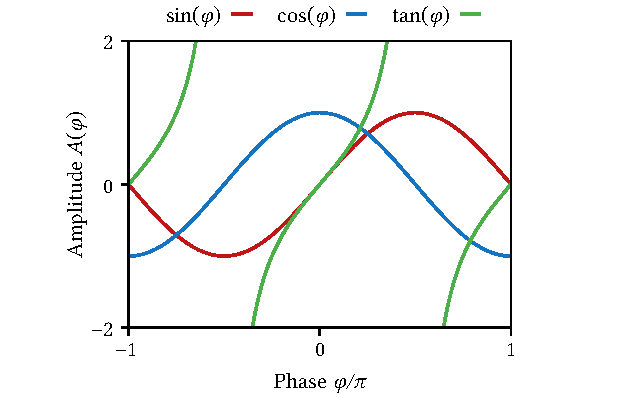
\includegraphics[width=0.2\textwidth]{test.jpg}
  \caption{This is simply a test figure, and equation $\sin(2x)=1$, and some SI unit \SI{1.0e3}{m/s}, and some chemical \ce{CrO2}. This text can even be made even longer, since we want to test this properly.}
  \label{fig:test}
\end{figure}


Morbi non tortor volutpat, mattis odio at, tincidunt libero.
Donec pulvinar et mi at varius.
Sed vulputate lectus eu libero gravida, vel porta tortor bibendum.
Quisque dictum ex id quam ultrices, ut commodo nisl euismod.
Aliquam vulputate, urna quis sodales rhoncus, orci metus pulvinar velit, feugiat sollicitudin dui massa interdum tortor.
Nam sed ante vitae eros imperdiet bibendum.
Fusce pretium semper leo eget lobortis.
Sed dictum erat quis diam faucibus bibendum.
Integer vitae enim euismod, ornare augue quis, pharetra ante.
Phasellus venenatis tellus ut velit faucibus, posuere porttitor lacus hendrerit.

\begin{table}[h!]
  \centering
  \caption{This is simply a test table.}
  \label{tab:test}
  \begin{tabular*}{\dimexpr\textwidth-4em\relax}{@{\extracolsep{\stretch{1}}\,}lcc@{\,}}
    \toprule
    Name    &   Symbol    &   Value             \\
    \midrule
    Euler constant          & $e$   & $2.71...$  \\
    Circle constant         & $\pi$ & $3.14...$ \\
    Imaginary identity      & $i$ & $\sqrt{-1}$ \\
    \bottomrule
  \end{tabular*}
\end{table}

Lorem ipsum dolor sit amet, consectetur adipiscing elit.
Donec malesuada magna sem.
Fusce vitae lectus id magna convallis euismod.
Quisque viverra sollicitudin turpis, vel ultricies mauris dictum quis.
Praesent justo nunc, luctus in lectus in, placerat tempus orci.
Donec placerat neque ac tortor dignissim pellentesque.
Aenean tellus erat, eleifend id interdum a, volutpat et massa.
Quisque tristique accumsan efficitur.

Morbi non tortor volutpat, mattis odio at, tincidunt libero.
Donec pulvinar et mi at varius.
Sed vulputate lectus eu libero gravida, vel porta tortor bibendum.
Quisque dictum ex id quam ultrices, ut commodo nisl euismod.
Aliquam vulputate, urna quis sodales rhoncus, orci metus pulvinar velit, feugiat sollicitudin dui massa interdum tortor.
Nam sed ante vitae eros imperdiet bibendum.
Fusce pretium semper leo eget lobortis.
Sed dictum erat quis diam faucibus bibendum.
Integer vitae enim euismod, ornare augue quis, pharetra ante.
Phasellus venenatis tellus ut velit faucibus, posuere porttitor lacus hendrerit.

Lorem ipsum dolor sit amet, consectetur adipiscing elit.
Donec malesuada magna sem.
Fusce vitae lectus id magna convallis euismod.
Quisque viverra sollicitudin turpis, vel ultricies mauris dictum quis.
Praesent justo nunc, luctus in lectus in, placerat tempus orci.
Donec placerat neque ac tortor dignissim pellentesque.
Aenean tellus erat, eleifend id interdum a, volutpat et massa.
Quisque tristique accumsan efficitur.


\section{Continuation}
Morbi non tortor volutpat, mattis odio at, tincidunt libero.
Donec pulvinar et mi at varius.
Sed vulputate lectus eu libero gravida, vel porta tortor bibendum.
Quisque dictum ex id quam ultrices, ut commodo nisl euismod.
Aliquam vulputate, urna quis sodales rhoncus, orci metus pulvinar velit, feugiat sollicitudin dui massa interdum tortor.
Nam sed ante vitae eros imperdiet bibendum.
Fusce pretium semper leo eget lobortis.
Sed dictum erat quis diam faucibus bibendum.
Integer vitae enim euismod, ornare augue quis, pharetra ante.
Phasellus venenatis tellus ut velit faucibus, posuere porttitor lacus hendrerit.

Lorem ipsum dolor sit amet, consectetur adipiscing elit~\cite{feynman,statistics}\footnote{Testing footnotes}.
Donec malesuada magna sem.
Fusce vitae lectus id magna convallis euismod.
Quisque viverra sollicitudin turpis, vel ultricies mauris dictum quis.
Praesent justo nunc, luctus in lectus in, placerat tempus orci.
Donec placerat neque ac tortor dignissim pellentesque.
Aenean tellus erat, eleifend id interdum a, volutpat et massa.
Quisque tristique accumsan efficitur.

Morbi non tortor volutpat, mattis odio at, tincidunt libero.
Donec pulvinar et mi at varius.
Sed vulputate lectus eu libero gravida, vel porta tortor bibendum.
Quisque dictum ex id quam ultrices, ut commodo nisl euismod.
Aliquam vulputate, urna quis sodales rhoncus, orci metus pulvinar velit, feugiat sollicitudin dui massa interdum tortor\footnote{This is another footnote test.; This is simply just a simple test, with an equation $\sin \alpha = \cos(2a-1)/\cos(2a+1)$. And here is a chemical element \ce{CrO23} and physical unit \SI{12e3}{m}.; Here is another footnote, also set in sans-serif.}.
Nam sed ante vitae eros imperdiet bibendum. 
Fusce pretium semper leo eget lobortis.
Sed dictum erat quis diam faucibus bibendum.
Integer vitae enim euismod, ornare augue quis, pharetra ante.
Phasellus venenatis tellus ut velit faucibus, posuere porttitor lacus hendrerit.

Lorem ipsum dolor sit amet, consectetur adipiscing elit.
Donec malesuada magna sem.
Fusce vitae lectus id magna convallis euismod.
Quisque viverra sollicitudin turpis, vel ultricies mauris dictum quis.
Praesent justo nunc, luctus in lectus in, placerat tempus orci.
Donec placerat neque ac tortor dignissim pellentesque.
Aenean tellus erat, eleifend id interdum a, volutpat et massa.
Quisque tristique accumsan efficitur.

Morbi non tortor volutpat, mattis odio at, tincidunt libero.
Donec pulvinar et mi at varius.
Sed vulputate lectus eu libero gravida, vel porta tortor bibendum.
Quisque dictum ex id quam ultrices, ut commodo nisl euismod.
Aliquam vulputate, urna quis sodales rhoncus, orci metus pulvinar velit, feugiat sollicitudin dui massa interdum tortor.
Nam sed ante vitae eros imperdiet bibendum.
Fusce pretium semper leo eget lobortis.
Sed dictum erat quis diam faucibus bibendum~\cite{particle}\footnote{Test}.
Integer vitae enim euismod, ornare augue quis, pharetra ante.
Phasellus venenatis tellus ut velit faucibus, posuere porttitor lacus hendrerit.


%
%\clearpage
%\chapter*{Bestemte integral}\noindent
%Under skal jeg prøve å gi en rask intro til bestemt integrasjon.
%Måten jeg gjør det på, er som følger: jeg kommer bare til å hoppe rett inn i det ved å demonstrere hvordan man løser to eksempeloppgaver.
%Etter det, skal jeg prøve å gi en kort oppsummering av hvordan man logisk kan tenke på bestemte integraler etterpå.
%Dette blir ikke en veldig dyp intro, men håper at det gir deg det du trenger for å løse eksamensoppgavene iallefall :).
%
%\section*{Eksempel I: introduksjon}\noindent
%La oss starte med et relativt enkelt eksempel på et bestemt integral:
%\begin{equation*}
%  \int_{x=0}^{x=1} x^2\,\text{d}x
%\end{equation*}
%Dette skrives ofte uten $x=\cdots$, altså på kortformen:
%\begin{equation*}
%  \int_{0}^{1} x^2\,\text{d}x
%\end{equation*}
%Når man skal løse et bestemt integral, må man alltid starte med å løse det ubestemte integralet.
%Hvis du slår opp i formelsamlingen bakerst i et av eksamenssettene, finner du en formel for ubestemte integral av polynomer:
%\begin{align*}
%  \int x^r\;\text{d}x &= \frac{1}{r+1} x^{r+1} & &\text{(for $r\neq-1$)}
%\end{align*}
%Setter du inn $r=2$ finner du da:
%\begin{align*}
%  \int x^2\;\text{d}x = \frac{1}{3} x^3
%\end{align*}
%Okay, la oss nå gå tilbake til det \emph{bestemte} integralet.
%Den vanlige måten å skrive ned at man har løst det \emph{ubestemte} integralet på, er å sette firkantklammer rundt svaret, med de såkallte \emph{integrasjonsgrensene} 0 og 1 utenfor klammene:
%\begin{equation*}
%  \int_{x=0}^{x=1} x^2\,\text{d}x = \left[ \frac{1}{3} x^3 \right]_{x=0}^{x=1}
%\end{equation*}
%Det å faktisk regne ut det bestemte integralet fra det ubestemte er nå veldig enkelt: vi trenger faktisk bare å sette inn $x=1$ og $x=0$ i det uttrykket som står i klammer, og så trekke svarene fra hverandre:
%\begin{align*}
%  \left[ \frac{1}{3} x^3 \right]_{x=0}^{x=1} 
%  &= \left[ \frac{1}{3} x^3 \right]_{x=1} - \;\;\;\;\left[ \frac{1}{3} x^3 \right]_{x=0} \\
%  &= \left[ \frac{1}{3} \cdot 1^3 \right]\;\;\; - \;\;\;\left[ \frac{1}{3} \cdot 0^3 \right] \\
%  &= \frac{1}{3} - 0 \\
%  &= \frac{1}{3}
%\end{align*}
%Svaret fra den bestemte integrasjonen blir altså:
%\begin{equation*}
%  \int_0^1 x^2\,\text{d}x = \frac{1}{3}
%\end{equation*}
%
%\section*{Eksempel II: avansert}
%Okay, la oss se på en litt mer avansert oppgave:
%\begin{equation*}
%  \int_1^\infty e^{-2x}
%\end{equation*}
%Første steg er som sagt alltid å løse det ubestemte integralet. 
%Sjekker du formelsamlingen bakerst i et eksamenssett dine, finner du denne likningen:
%\begin{align*}
%  \int e^{kx}\;\text{d}x &= \frac{1}{k} e^{kx} + C & &\text{($C$ er en vilkårlig konstant)}
%\end{align*}
%Sett inn at $k=-2$:
%\begin{align*}
%  \int e^{-2x}\;\text{d}x &= -\frac{1}{2} e^{-2x} + C
%\end{align*}
%Så løsningen på det ubestemte integralet er også:
%\begin{align*}
%  \int_{1}^{\infty} e^{-2x}\;\text{d}x &= \left[ -\frac{1}{2} e^{-2x} + C \right]_1^\infty
%\end{align*}
%Vi finner da løsningen på det bestemte integralet ved å sette inn $x=\infty$ og $x=1$, og trekke resultatene fra hverandre.
%En detalj som trengs her, er da at $e^{-\infty} = 1/e^{\infty} = 1/\infty = 0$; har du ikke lært om grenseverdier i faget, så trenger du ikke å tenke så mye på dette, det er isåfall muligens utenfor pensum :).
%Men beregningen blir altså:
%\begin{align*}
%  \int_{1}^{\infty} e^{-2x}\;\text{d}x 
%  &= \left[ -\frac{1}{2} e^{-2x}     + C \right]_1^\infty \\
%  &= \left[ -\frac{1}{2} e^{-2x}     + C \right]_{x=\infty} - \;\;\;\;\left[ -\frac{1}{2} e^{-2x} + C \right]_{x=1} \\
%  &= \left[ -\frac{1}{2} e^{-\infty} + C \right] \;\;\;\;\;\; - \;\;\;\; \left[ -\frac{1}{2} e^{-2} + C \right] \\
%  &= \left[ -\frac{1}{2} \cdot 0 \; +  C \right] \;\;\;\;\;\; - \;\;\;\; \left[ -\frac{1}{2} e^{-2} + C \right] \\
%  &= 0 + C + \frac{1}{2} e^{-2} - C \\
%  &= \frac{1}{2} e^{-2} \\
%  &= \frac{1}{2e^2}
%\end{align*}
%Så svaret er:
%\begin{align*}
%  \int_{1}^{\infty} e^{-2x}\;\text{d}x &= \frac{1}{2e^2}
%\end{align*}
%Merk at det ikke hadde noe å si at vi ikke visste hva den ukjente konstanten $C$ var for noe, den forsvant uansett når vi beregnet et bestemt integral :).
%
%\section*{Tolkning I: antiderivasjon}
%En måte å tolke hva integrasjon betyr for noe, er at det er \emph{det omvendte av derivasjon}. 
%For eksempel, hvis vi tar det ubestemte integralet vi så på over:
%\begin{align*}
%  \int x^2\;\text{d}x &= \frac{1}{3} x^{3}
%\end{align*}
%Hva skjer hvis vi deriverer svaret? 
%Jo, den deriverte av $x^{3}$ er $3x^2$, så vi får:
%\begin{align*}
%  \left( \int x^2\;\text{d}x \right)' &= x^{2}
%\end{align*}
%Så hvis vi først integrerer $x^2$ og så deriverer svaret, så får vi tilbake det vi startet med.
%Derivasjonen gjorde det motsatte av det integrasjonen gjorde.
%
%Hva betyr dette for hvordan vi skal tolke integrasjon?
%Jo, det derivasjon måler er jo \emph{stigningstallet} eller \emph{endringsraten} til noe.
%For eksempel, hvis du vet posisjonen $s$ til en bil som funksjon av tiden $t$, så vil den deriverte $v(t) = s'(t)$ være \emph{hastigheten} til bilen.
%Siden integrasjon gjør det motsatte, betyr det at du kan integrere hastigheten for å finne ut hvor langt bilen faktisk har kjørt.
%
%
%\section*{Tolkning II: areal under en kurve}
%En geometrisk tolkning av integrasjon, er at det er en måte å regne ut arealet under en kurve.
%La oss f.eks. si at vi har en graf av funksjonen $f(x) = 1-x^2$:\\
%{\quad \includegraphics[width=0.6\textwidth]{/home/jabirali/figure.png}} \\
%Hvis vi tar et bestemt integral av denne funksjonen fra $x=0$ til $x=1$:
%\begin{equation*}
%  \int_0^1 (1-x^2)\;\text{d}x = \left[ x - \frac{1}{3}x^3 \right]_0^1 = [1 - 1/3] - [0 - 0] = 2/3
%\end{equation}
%Egentlig bare arealet under kurven mellom $x=0$ og $x=1$:\\
%{\quad \includegraphics[width=0.6\textwidth]{/home/jabirali/areal.png}}\\
%Det å \emph{bevise} at integraler gir deg areal er litt mer jobb, og sannsynligvis ikke verdt å fokusere på fram mot eksamen.
%Men det er greit å ha i bakhodet at hvis det kommer en eksamensoppgave hvor de vil at du skal ``finne arealet under kurven'', så betyr det bare at du skal løse et bestemt integral ;).
%
%Det at ``integral'' betyr ``areal under kurve'' gir jo en innsikt til.
%Et ``bestemt integral fra $x=0$ til $x=1$'' er altså arealet under kurven mellom punktene $x=0$ og $x=1$.
%Et ``ubestemt integral'' derimot, hvor vi ikke har satt inn noen verdier for $x$ enda, er en generell formel for å regne ut arealet under kurven for vilkårlige startpunkt og sluttpunkt.
%Dette minner jo litt om den samme situasjonen for derivasjon: $f'(x)$ er en ``ubestemt derivert'', altså en generell formel for å regne ut stigningstall. Hvis du setter inn $x=2$ i dette uttrykket, altså beregner $f'(2)$, så har du derimot spesifikt stigningstallet til kurven i punktet $x=2$, som vi godt kunne kallt en ``bestemt derivert''.




